% !TEX TS-program = xelatex
% !BIB program = bibtex
% !TeX spellcheck = ru_RU

% About magic macroses see also
% https://tex.stackexchange.com/questions/78101/

% По умолчанию используется шрифт 14 размера. Если нужен 12-й шрифт, уберите опцию [14pt]
\documentclass[14pt
  , russian
  %, xcolor={svgnames}
  ]{matmex-diploma-custom}
\usepackage[table]{xcolor}
\usepackage{graphicx}
\usepackage{tabularx}
\newcolumntype{Y}{>{\centering\arraybackslash}X}
\usepackage{amsmath}
\usepackage{amsthm}
\usepackage{amsfonts}
\usepackage{amssymb}
\usepackage{mathtools}
\usepackage{thmtools}
\usepackage{thm-restate}
\usepackage{tikz}
\usepackage{wrapfig}
% \usepackage[kpsewhich,newfloat]{minted}
% \usemintedstyle{vs}
\usepackage[inline]{enumitem}
\usepackage{subcaption}
\usepackage{caption}
\usepackage[nocompress]{cite}
\usepackage{makecell}
% \setitemize{noitemsep,topsep=0pt,parsep=0pt,partopsep=0pt}
% \setenumerate{noitemsep,topsep=0pt,parsep=0pt,partopsep=0pt}


\graphicspath{ {resources/} }

% 
% % \documentclass 
% %   [ a4paper        % (Predefined, but who knows...)
% %   , draft,         % Show bad things.
% %   , 12pt           % Font size.
% %   , pagesize,      % Writes the paper size at special areas in DVI or
% %                    % PDF file. Recommended for use.
% %   , parskip=half   % Paragraphs: noindent + gap.
% %   , numbers=enddot % Pointed numbers.
% %   , BCOR=5mm       % Binding size correction.
% %   , submission
% %   , copyright
% %   , creativecommons 
% %   ]{eptcs}
% % \providecommand{\event}{ML 2018}  % Name of the event you are submitting to
% % \usepackage{breakurl}             % Not needed if you use pdflatex only.
% 
% \usepackage{underscore}           % Only needed if you use pdflatex.
% 
% \usepackage{booktabs}
% \usepackage{amssymb}
% \usepackage{amsmath}
% \usepackage{mathrsfs}
% \usepackage{mathtools}
% \usepackage{multirow}
% \usepackage{indentfirst}
% \usepackage{verbatim}
% \usepackage{amsmath, amssymb}
% \usepackage{graphicx}
% \usepackage{xcolor}
% \usepackage{url}
% \usepackage{stmaryrd}
% \usepackage{xspace}
% \usepackage{comment}
% \usepackage{wrapfig}
% \usepackage[caption=false]{subfig}
% \usepackage{placeins}
% \usepackage{tabularx}
% \usepackage{ragged2e}
% \usepackage{soul}
\usepackage{csquotes}
% \usepackage{inconsolata}
% 
% \usepackage{polyglossia}   % Babel replacement for XeTeX
%   \setdefaultlanguage[spelling=modern]{russian}
%   \setotherlanguage{english}
% \usepackage{fontspec}    % Provides an automatic and unified interface 
%                          % for loading fonts.
% \usepackage{xunicode}    % Generate Unicode chars from accented glyphs.
% \usepackage{xltxtra}     % "Extras" for LaTeX users of XeTeX.
% \usepackage{xecyr}       % Help with Russian.
% 
% %% Fonts
% \defaultfontfeatures{Mapping=tex-text}
% \setmainfont{CMU Serif}
% \setsansfont{CMU Sans Serif}
% \setmonofont{CMU Typewriter Text}

\usepackage[final]{listings}

\lstdefinelanguage{ocaml}{
keywords={@type, function, fun, let, in, match, with, when, class, type,
nonrec, object, method, of, rec, repeat, until, while, not, do, done, as, val, inherit, and,
new, module, sig, deriving, datatype, struct, if, then, else, open, private, virtual, include, success, failure,
lazy, assert, true, false, end},
sensitive=true,
commentstyle=\small\itshape\ttfamily,
keywordstyle=\ttfamily\bfseries, %\underbar,
identifierstyle=\ttfamily,
basewidth={0.5em,0.5em},
columns=fixed,
fontadjust=true,
literate={->}{{$\to$}}3 {===}{{$\equiv$}}1 {=/=}{{$\not\equiv$}}1 {|>}{{$\triangleright$}}3 {\\/}{{$\vee$}}2 {/\\}{{$\wedge$}}2 {>=}{{$\ge$}}1 {<=}{{$\le$}} 1,
morecomment=[s]{(*}{*)}
}

\lstset{
mathescape=true,
%basicstyle=\small,
identifierstyle=\ttfamily,
keywordstyle=\bfseries,
commentstyle=\scriptsize\rmfamily,
basewidth={0.5em,0.5em},
fontadjust=true,
language=ocaml
}
 
\newcommand{\cd}[1]{\texttt{#1}}
\newcommand{\inbr}[1]{\left<#1\right>}


\newcolumntype{L}[1]{>{\raggedright\let\newline\\\arraybackslash\hspace{0pt}}m{#1}}
\newcolumntype{C}[1]{>{\centering\let\newline\\\arraybackslash\hspace{0pt}}m{#1}}
\newcolumntype{R}[1]{>{\raggedleft\let\newline\\\arraybackslash\hspace{0pt}}m{#1}}



\usepackage{soul}
\usepackage[normalem]{ulem}
%\sout{Hello World}

% перевод заголовков в листингах
\renewcommand\lstlistingname{Листинг}
\renewcommand\lstlistlistingname{Листинги}

\usepackage{afterpage}
\usepackage{pdflscape}
% TODO: Понять, почему я выделил то, что тут в отдельный файл
\usepackage{listings}
\usepackage{tikz}
\usetikzlibrary{decorations.pathreplacing,calc,shapes,positioning,tikzmark}

\newcounter{tmkcount}

\tikzset{
  use tikzmark/.style={
    remember picture,
    overlay,
    execute at end picture={
      \stepcounter{tmkcount}
    },
  },
  tikzmark suffix={-\thetmkcount}
}

\usepackage{totcount}

\usepackage{caption}
\usepackage{listings}
\usepackage{minted}

\RecustomVerbatimEnvironment{Verbatim}{BVerbatim}{}

\renewcommand{\figurename}{Listing}

\DeclareCaptionFont{white}{ \color{white} }
\DeclareCaptionFormat{listing}{
    \parbox{\textwidth}{\hspace{15pt}#1#2#3}
}

\newcommand\todo[1]{{\color{violet}#1}}
\newcommand\db[1]{{\color{red}#1}}
\newcommand\question[1]{{\color{cyan}#1}}

% color for tables
\usepackage{colortbl}
% define new colors
\definecolor{LightRed}{RGB}{204, 230, 255}
\definecolor{LightBlue}{RGB}{140,186,252}

\definecolor{forestgreen(web)}{rgb}{0.13, 0.55, 0.13}
% use the colortbl package to define a new column
\newcolumntype{a}{>{\columncolor{LightRed}}c}

\usepackage{multirow}
 
 
\definecolor{codegreen}{rgb}{0,0.6,0}
\definecolor{codegray}{rgb}{0.5,0.5,0.5}
\definecolor{codepurple}{rgb}{0.58,0,0.82}
\definecolor{backcolour}{rgb}{0.95,0.95,0.92}


\usepackage[font=small,labelfont=bf]{caption} % Required for specifying captions to tables and figures

\begin{document}
%% Если что-то забыли, при компиляции будут ошибки Undefined control sequence \my@title@<что забыли>@ru
%% Если англоязычная титульная страница не нужна, то ее можно просто удалить.
\filltitle{ru}{
    %% Актуально только для курсовых/практик. ВКР защищаются не на кафедре а в ГЭК по направлению, 
    %%   и к моменту защиты вы будете уже не в группе.
    chair              = {Кафедра системного программирования},
    group              = {19Б.10-мм},
    %
    %% Макрос filltitle ненавидит пустые строки, поэтому обязателен хотя бы символ комментария на строке
    %% Актуально всем.
    title              = {Разработка алгоритма для задачи достижимости с регулярными ограничениями},
    % 
    %% Здесь указывается тип работы. Возможные значения:
    %%   coursework - отчёт по курсовой работе;
    %%   practice - отчёт по учебной практике;
    %%   prediploma - отчёт по преддипломной практике;
    %%   master - ВКР магистра;
    %%   bachelor - ВКР бакалавра.
    type               = {practice},
    %
    %% Здесь указывается вид работы. От вида работы зависят критерии оценивания.
    %%   solution - <<Решение>>. Обучающемуся поручили найти способ решения проблемы в области разработки программного обеспечения или теоретической информатики с учётом набора ограничений.
    %%   experiment - <<Эксперимент>>. Обучающемуся поручили изучить возможности, достоинства и недостатки новой технологии, платформы, языка и т. д. на примере какой-то задачи.
    %%   production - <<Производственное задание>>. Автору поручили реализовать потенциально полезное программное обеспечение.
    %%   comparison - <<Сравнение>>. Обучающемуся поручили сравнить несколько существующих продуктов и/или подходов.
    %%   theoretical - <<Теоретическое исследование>>. Автору поручили доказать какое-то утверждение, исследовать свойства алгоритма и т.п., при этом не требуя написания кода.
    kind               = {solution},
    %
    author             = {Порсев Денис Витальевич},
    % 
    %% Актуально только для ВКР. Указывается код и название направления подготовки. Типичные примеры:
    %%   02.03.03 <<Математическое обеспечение и администрирование информационных систем>>
    %%   02.04.03 <<Математическое обеспечение и администрирование информационных систем>>
    %%   09.03.04 <<Программная инженерия>>
    %%   09.04.04 <<Программная инженерия>>
    %% Те, что с 03 в середине --- бакалавриат, с 04 --- магистратура.
    specialty          = {02.03.03 <<Математическое обеспечение и администрирование информационных систем>>},
    % 
    %% Актуально только для ВКР. Указывается шифр и название образовательной программы. Типичные примеры:
    %%   СВ.5006.2017 <<Математическое обеспечение и администрирование информационных систем>>
    %%   СВ.5162.2020 <<Технологии программирования>>
    %%   СВ.5080.2017 <<Программная инженерия>>
    %%   ВМ.5665.2019 <<Математическое обеспечение и администрирование информационных систем>>
    %%   ВМ.5666.2019 <<Программная инженерия>>
    %% Шифр и название программы можно посмотреть в учебном плане, по которому вы учитесь. 
    %% СВ.* --- бакалавриат, ВМ.* --- магистратура. В конце --- год поступления (не обязательно ваш, если вы были в академе/вылетали).
    programme          = {СВ.5006.2017 <<Математическое обеспечение и администрирование информационных систем>>},
    % 
    %% Актуально только для ВКР, только для матобеса и только 2017-2018 годов поступления. Указывается профиль подготовки, на котором вы учитесь.
    %% Названия профилей можно найти в учебном плане в списке дисциплин по выбору. На каком именно вы, вам должны были сказать после второго курса (можно уточнить в студотделе).
    %% Вот возможные вариканты:
    %%   Математические основы информатики
    %%   Информационные системы и базы данных
    %%   Параллельное программирование
    %%   Системное программирование
    %%   Технология программирования
    %%   Администрирование информационных систем
    %%   Реинжиниринг программного обеспечения
    % profile            = {Системное программирование},
    % 
    %% Актуально всем.
    %supervisorPosition = {проф. каф. СП, д.ф.-м.н., проф.}, % Терехов А.Н.
    supervisorPosition = {доцент кафедры информатики, к.ф.-м.н.,}, % Григорьев С.В.
    supervisor         = {Григорьев С.В.}
    % 

    % consultantPosition = {должность ООО <<Место работы>> степень},
    % consultant         = {К.К. Консультант}
}

\maketitle
\setcounter{tocdepth}{2}
\tableofcontents


% У введения нет номера главы
\section{Introduction}

Scalable high-performance graph analysis is an actual challenge.
There is a big number of ways to attack this challenge~\cite{Coimbra2021} and the first promising idea is to utilize general-purpose graphic processing units (GPGPU-s).
Such existing solutions, as CuSha~\cite{10.1145/2600212.2600227} and Gunrock~\cite{7967137} show that utilization of GPUs can improve the performance of graph analysis, moreover it is shown that solutions may be scaled to multi-GPU systems.
But low flexibility and high complexity of API are problems of these solutions.

The second promising thing which provides a user-friendly API for high-performance graph analysis algorithms creation is a GraphBLAS API~\cite{7761646} which provides linear algebra based building blocks to create graph analysis algorithms.
The idea of GraphBLAS is based on is a well-known fact that linear algebra operations can be efficiently implemented on parallel hardware.
Along with this, a graph can be natively represented using matrices: adjacency matrix, incidence matrix, etc.
While reference CPU-based implementation of GraphBLAS, SuiteSparse:GraphBLAS~\cite{10.1145/3322125}, demonstrates good performance in real-world tasks, GPU-based implementation is challenging.

One of the challenges in this way is that real data are often sparse, thus underlying matrices and vectors are also sparse, and, as a result, classical dense data structures and respective algorithms are inefficient. 
So, it is necessary to use advanced data structures and procedures to implement sparse linear algebra, but the efficient implementation of them on GPU is hard due to the irregularity of workload and data access patterns.
Though such well-known libraries as cuSparse show that sparse linear algebra operations can be efficiently implemented for GPGPU-s, it is not so trivial to implement GraphBLAS on GPGPU. 
First of all, it requires \textit{generic} sparse linear algebra, thus it is impossible just to reuse existing libraries which are almost all specified for operations over floats.
The second problem is specific optimizations, such as maskings fusion, which can not be natively implemented on top of existing kernels.
Nevertheless, there is a number of implementations of GraphBLAS on GPGPU, such as GraphBLAST:~\cite{yang2019graphblast}, GBTL~\cite{7529957}, which show that GPGPUs utilization can improve the performance of GraphBLAS-based graph analysis solutions.
But these solutions are not portable because they are based on Nvidia Cuda stack.
Moreover, the scalability problem is not solved: all these solutions support only single-GPU, not multi-GPU computations.

To provide portable GPU implementation of GraphBLAS API we developed a \textit{SPLA} library (sources are published on GitHub: \url{https://github.com/JetBrains-Research/spla}).
This library utilizes OpenCL for GPGPU computing to be portable across devices of different vendors.
Moreover, it is initially designed to utilize multiple GPGPUs to be scalable.
To sum up, the contribution of this work is the following.
\begin{itemize}
    \item Design of portable GPU GraphBLAS implementation proposed. The design involves the utilization of multipole GPUS. Additionally, the proposed design is aimed to simplify library tuning and wrappers for different high-level platforms and languages creation. 
    \item Subset of GraphBLAS API, including such operations as masking, matrix-matrix multiplication, matrix-matrix e-wise addition, is implemented. The current implementation is limited by COO and CSR matrix representation format and uses basic algorithms for some operations, but work in progress and more data formats will be supported and advanced algorithms will be implemented in the future.
    \item Preliminary evaluation on such algorithms as breadth-first search (BFS) and triangles counting (TC), and real-world graphs shows portability across different vendors and promising performance: for some problems Spla is comparable with GraphBLAST. Surprisingly, for some problems, the proposed solution on embedded Intel graphic card shows better performance than SuiteSparse:GraphBLAS on the same CPU. At the same time, the evaluation shows that further optimization is required.
\end{itemize} 
\section*{Problem statement}
The aim of this work is to evaluate whether it is practical and effective to utilize distillation and specialized hardware to optimize programs that contain sparse linear algebra routines. The work elaborates on distillation and high-level synthesis, outlining key challenges to obtain a better solution. In order to achieve the aim, the following objectives were set.
\begin{itemize}
    \item Study approaches for providing fusion in different areas.
    \item Implement hardware generation with fusion in mind.
    \item Design memory interface.
    \item Implement the testbench and carry out the evaluation.
\end{itemize}
\section{Background}
\label{sec:background}
\subsection{CFL-reachability}

\subsection{Recursive State Machines}
In this work we use the notion of \textit{Finite-State Machine} (FSM).

\begin{definition}
A \textit{deterministic finite-state machine without $\varepsilon$-transitions} $T$ is a tuple $\langle \Sigma, Q, Q_s, Q_f, \delta \rangle$, where:
\begin{itemize}
    \item $\Sigma$ is an input alphabet,
    \item $Q$ is a finite set of states,
    \item $Q_s \subseteq Q$ is a set of start (or initial) states,
    \item $Q_f \subseteq Q$ is a set of final states,
    \item $\delta: Q \times \Sigma \to Q$ is a transition function.
\end{itemize}
\end{definition}

It is well known, that every regular expression can be converted to deterministic FSM without $\varepsilon$-transitions~\cite{automata:theory:10.5555/1177300}.

While a regular expression can be transformed to an FSM, a context-free grammar can be transformed to a \textit{Recursive State Machine} (RSM) in a similar fashion.
In our work, we use the following definition of RSM based
on~\cite{rsm:analysis:10.1007/3-540-44585-4_18}.

\begin{definition}
A \textit{recursive state machine} $R$ over a finite alphabet $\Sigma$ is defined as a tuple of elements $\langle B,m,\{C_i\}_{i \in B} \rangle$, where:

\begin{itemize}
    \item $B$ is a finite set of labels of boxes,
    \item $m \in B$ is an initial box label,
    \item Set of \textit{component state machines} or \textit{boxes},
          where $C_i=(\Sigma \cup B, Q_i,q_i^0,F_i,\delta_i)$:
    \begin{itemize}
        \item $\Sigma \cup B$ is a set of symbols, $\Sigma \cap B = \varnothing$,
        \item $Q_i$ is a finite set of states,
              where $Q_i \cap Q_j =  \varnothing, \forall i \neq j$,
        \item $q_i^0$ is an initial state for $C_i$,
        \item $F_i$ is a set of final states for $C_i$, where $F_i \subseteq Q_i$,
        \item $\delta_i: Q_i \times (\Sigma \cup B) \to Q_i$ is a transition function. %for $C_i$
    \end{itemize}
\end{itemize}

\end{definition}

\begin{definition}
    The \textit{size of RSM} $|R|$ is defined as the sum of the number of states in all boxes.
\end{definition}

RSM behaves as a set of finite state machines (or FSM).
Each such FSM is called a \textit{box} or a \textit{component state machine}.
A box works similarly to the classic FSM, but it also handles additional \textit{recursive calls} and employs an implicit \textit{call stack} to \textit{call} one component from another and then return execution flow back.

\subsection{Linear algebra}
\paragraph*{Graph Kronecker product and machines intersection}
\begin{definition}
Given two matrices $A$ and $B$ of sizes $m_1 \times n_1$ and $m_2 \times n_2$
respectively, with element-wise product operation $\cdot$, the Kronecker product of these two matrices is a new matrix $C = A \otimes B$ of size $m_1 * m_2 \times n_1 * n_2$ and \[C[u * m_2 + v,n_2 * p + q] = A[u,p] \cdot B[v,q].\]
\end{definition}
\begin{definition}
\label{def:graph:product}
Given two edge-labeled directed graphs $\mathcal{G}_1=\langle V_1, E_1, L_1 \rangle$
and $\mathcal{G}_2=\langle V_2, E_2, L_2 \rangle$,
the \textit{Kronecker product} of these two graphs is a edge-labeled directed graph
$\mathcal{G}=\mathcal{G}_1 \otimes \mathcal{G}_2$,
where $\mathcal{G}= \langle V, E, L \rangle$:
\begin{itemize}
    \item $V = V_1 \times V_2$
    \item $E = \{((u,v),l,(p,q)) \mid (u,l,p) \in E_1 \wedge (v,l,q) \in E_2 \}$
    \item $L = L_1 \cap L_2$
\end{itemize}
\end{definition}

The Kronecker product for graphs produces a new graph with a property
that if and only if some path $(u,v)\pi(p,q)$ exists in the result graph
then paths $u\pi_1p$ and $v\pi_2q$ exist in the input graphs,
and $\omega(\pi) = \omega(\pi_1) = \omega(\pi_2)$.
These paths $\pi_1$ and $\pi_2$ can easily be found from $\pi$ by its definition.

The Kronecker product for directed graphs can be described as
the Kronecker product of the corresponding adjacency matrices of graphs,
what gives the following definition:

\begin{definition}
\label{def:graph:adjproduct}
Given two adjacency matrices $M_1$ and $M_2$ of sizes
$m_1 \times n_1$ and $m_2 \times n_2$ respectively
for some directed graphs $\mathcal{G}_1$ and $\mathcal{G}_2$,
the \textit{Kronecker product} of these two adjacency matrices is the adjacency matrix $M$
of some graph $\mathcal{G}$, where $M$ has size $m_1 * m_2 \times n_1 * n_2$ and
\[M[u * m_2 + v,n_2 * p + q] = M_1[u,p] \cap M_2[v,q].\]
\end{definition}

By definition, the Kronecker product for adjacency matrices gives an
adjacency matrix with the same set of edges as in the resulting graph in the
Definition~\ref{def:graph:product}. Thus, $M(\mathcal{G}) = M(\mathcal{G}_1) \otimes
M(\mathcal{G}_2)$, where $\mathcal{G} = \mathcal{G}_1 \otimes \mathcal{G}_2$.

\begin{definition}
\label{def:fsm:intersection}
Given two finite state machines 
$T_1 = \langle \Sigma, Q^1, Q_S^1, Q_F^1, \delta^1 \rangle$ and \\
$T_2 = \langle \Sigma, Q^2, Q_S^2, Q_F^2, \delta^2 \rangle$, the \textit{intersection} of these two machines is a new FSM $T = \langle \Sigma, Q, Q_S, Q_F, \delta \rangle$, where:
\begin{itemize}
    \item $Q = Q^1 \times Q^2$
    \item $Q_S = Q_S^1 \times Q_S^2$
    \item $Q_F = Q_F^1 \times Q_F^2$
    \item $\delta: Q \times \Sigma \to Q$,
    $\delta (\langle q_1, q_2 \rangle, s) = \langle q_1', q_2' \rangle$, if $\delta(q_1,s)=q_1'$ and $\delta(q_2,s)=q_2'$
\end{itemize}
\end{definition}

According to~\cite{automata:theory:10.5555/1177300} an FSM intersection defines the machine for which $L(T) = L(T_1) \cap L(T_2)$.



\subsection{Pointer analysis as CFL-reachability problem}
\paragraph*{Memory alias}

\paragraph*{Points-to analysis for Java}
\clearpage
\section{Specialized hardware generation with fusion}

As has already been mentioned, we utilize distillation to provide fusion for routines written in a simple functional programming language and utilize FHW compiler, which is able to translate any Haskell program into SystemVerilog and eventually into bitcode for  FPGA. This section discusses how the gap between the distiller language and Haskell was closed, what issues in FHW were found and how they were solved. Also the section describes data structures being used for which fusion via distillation works well.


\subsection{Distiller}

The distiller from~\cite{distillation} operates on programs written in \texttt{.pot} language: a simple call-by-name functional language. Its syntax resembles the one of Haskell, but it encloses the arguments of a constructor in parentheses and separates them with a comma to make parsing easier. In order to emit Haskell, the pretty-printer prints such constructors correspondingly and maintains correct indentation for case alternatives, which are originally separated by \texttt{|} in \texttt{.pot}. With such modifications, it is possible to emit Haskell code from \texttt{.pot} programs and eventually pass them into FHW compiler. It is worth noting that \texttt{.pot} assumes a Hindley-Milner type system, but its implementation is untyped; thus the emitted program should be extended by hand to contain proper type definitions and annotations where needed to eliminate unnecessary typeclasses.

Another issue is that the distiller originally produced duplicated functions during residualization. Such functions increase the size of the generated hardware significantly for reasonable examples and make translation into hardware more complex. The functions are filtered to contain only non-duplicates. Since functions use De Bruijn indexes for bound variables, functions are considered to be duplicates if their bodies are equal after we replace each recursive call in one function with the name of the other function.

\subsection{FHW}

Unlike~\cite{Edwards2019FHWP}, which utilized C++ Verilator simulation, we use Xilinx Vivado to both simulate the generated SystemVerilog and to synthesize it. It allows to better estimate design and memory transferring overheads.

Initially, generated hardware did not work in Vivado simulation due to the multiple driving of \texttt{initial} blocks, which are also not synthesizable. Such blocks were replaced with a \texttt{reset} signal. The dataflow network works under valid-ready protocol, and memory output had to be invalidated to prevent the propagation of undefined signals. Such outputs are invalidated on the positive edge of the reset signal.

After that, it appeared that the compiler could not handle examples with sparse linear algebra routines due to the limited maximum number (64) of inputs in merge actors. For each merge actor in the dataflow there is a sum datatype with the number of fields equal to the number of merge inputs to be able to correctly type each merge and to identify the chosen input to pass that choice to another actor: demux, fork or mux. Such datatypes are recursively split until every datatype satisfies the restriction. The inputs of a merge are also split and a new layer of merge actors is added on top, as it could be seen in figure~\ref{fig:compressChoice} where the limit is 2 while the original input size is 4; consuming actor is split accordingly. Similar procedure is applied for datatypes that arise during lowering passes of FHW, for example, if the defunctionalization pass introduces more than 64 constructors in the corresponding datatype. An example of such step could be seen in listing~\ref{lst:split}, if we suppose that maximum supported number of alternatives is 4.

\begin{listing}
\begin{center}
\begin{minted}{Haskell}

data Cont = C_1 | C_2 | C_3 | C_4
-- transformed into
data LeftCont = C_1 | C_2
data RightCont = C_3 | C_4
data Cont = LeftCont | RightCont

\end{minted}
\caption{Data type split step}
\label{lst:split}
\end{center}
\end{listing}


\begin{figure}
    \centering
    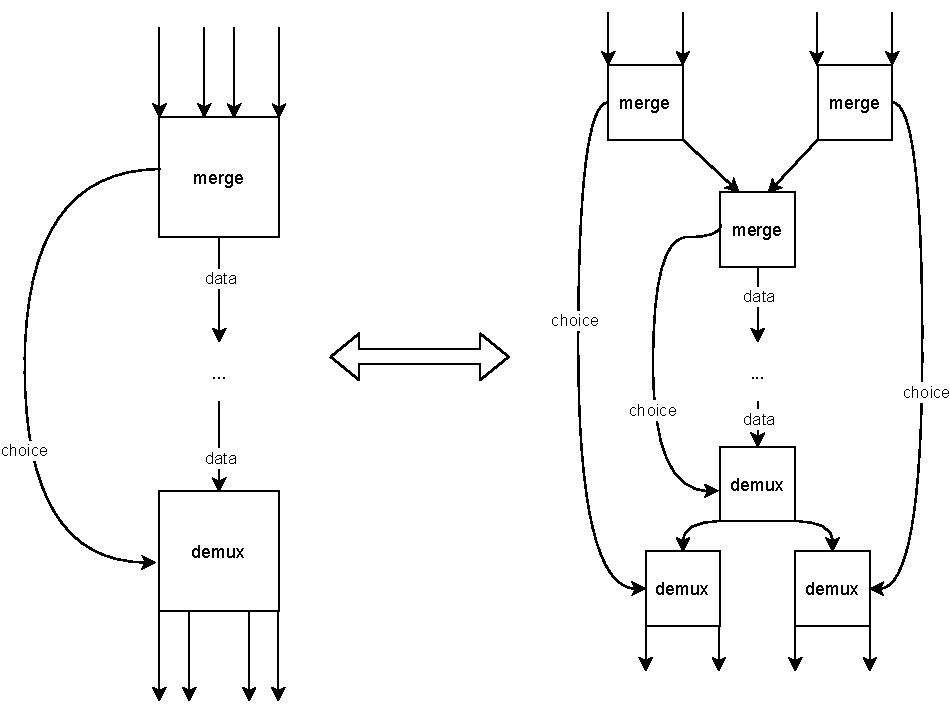
\includegraphics[width=0.8\textwidth]{figures/compressChoice.pdf}
    \caption{Merge split}
    \label{fig:compressChoice}
\end{figure}

\subsection{Data types}

The success of sparse linear algebra functions fusion depends on the compressed representation being used. Our choice here is quadtree representation~\cite{qtree}. It provides a reasonable compression rate compared to traditionally used formats, e.g., coordinate format, or compressed sparse row representation~\cite{GAILLA}, consuming 1.5x more memory on average in our experiments, although memory consumption grows logarithmically with the dimensions of a matrix. Also, it allows to express algorithms in a divide and conquer manner leaving indexing implicit, which facilitates fusion. The representation simply recursively splits the matrix into submatrices until the size of 1x1 or until the submatrix is empty. Thus it encodes only matrices with the size of power of 2, but any matrix could be extended with zeroes to fit the size requirement. An example of such representation could be seen in figure~\ref{fig:qtree}, where a matrix with 4 non-zero entries is depicted. Dashed squares represent either submatrix with only zero entries or zero entry. A procedure of getting a quadtree representation from coordinate format could be found in~\cite{matrix-rep}. Since the representation is constructive, it is possible to utilize dependent type programming techniques to, for example, specify correct by construction routines or use rewrite rules for matrix relations to optimize routines, following the approach of~\cite{typeyourmatricesforgreatgood}. Next, we use terms tree, quadtree or matrix interchangeably: they all mean a sparse matrix representation via quadtree. 

\begin{figure}
    \centering
    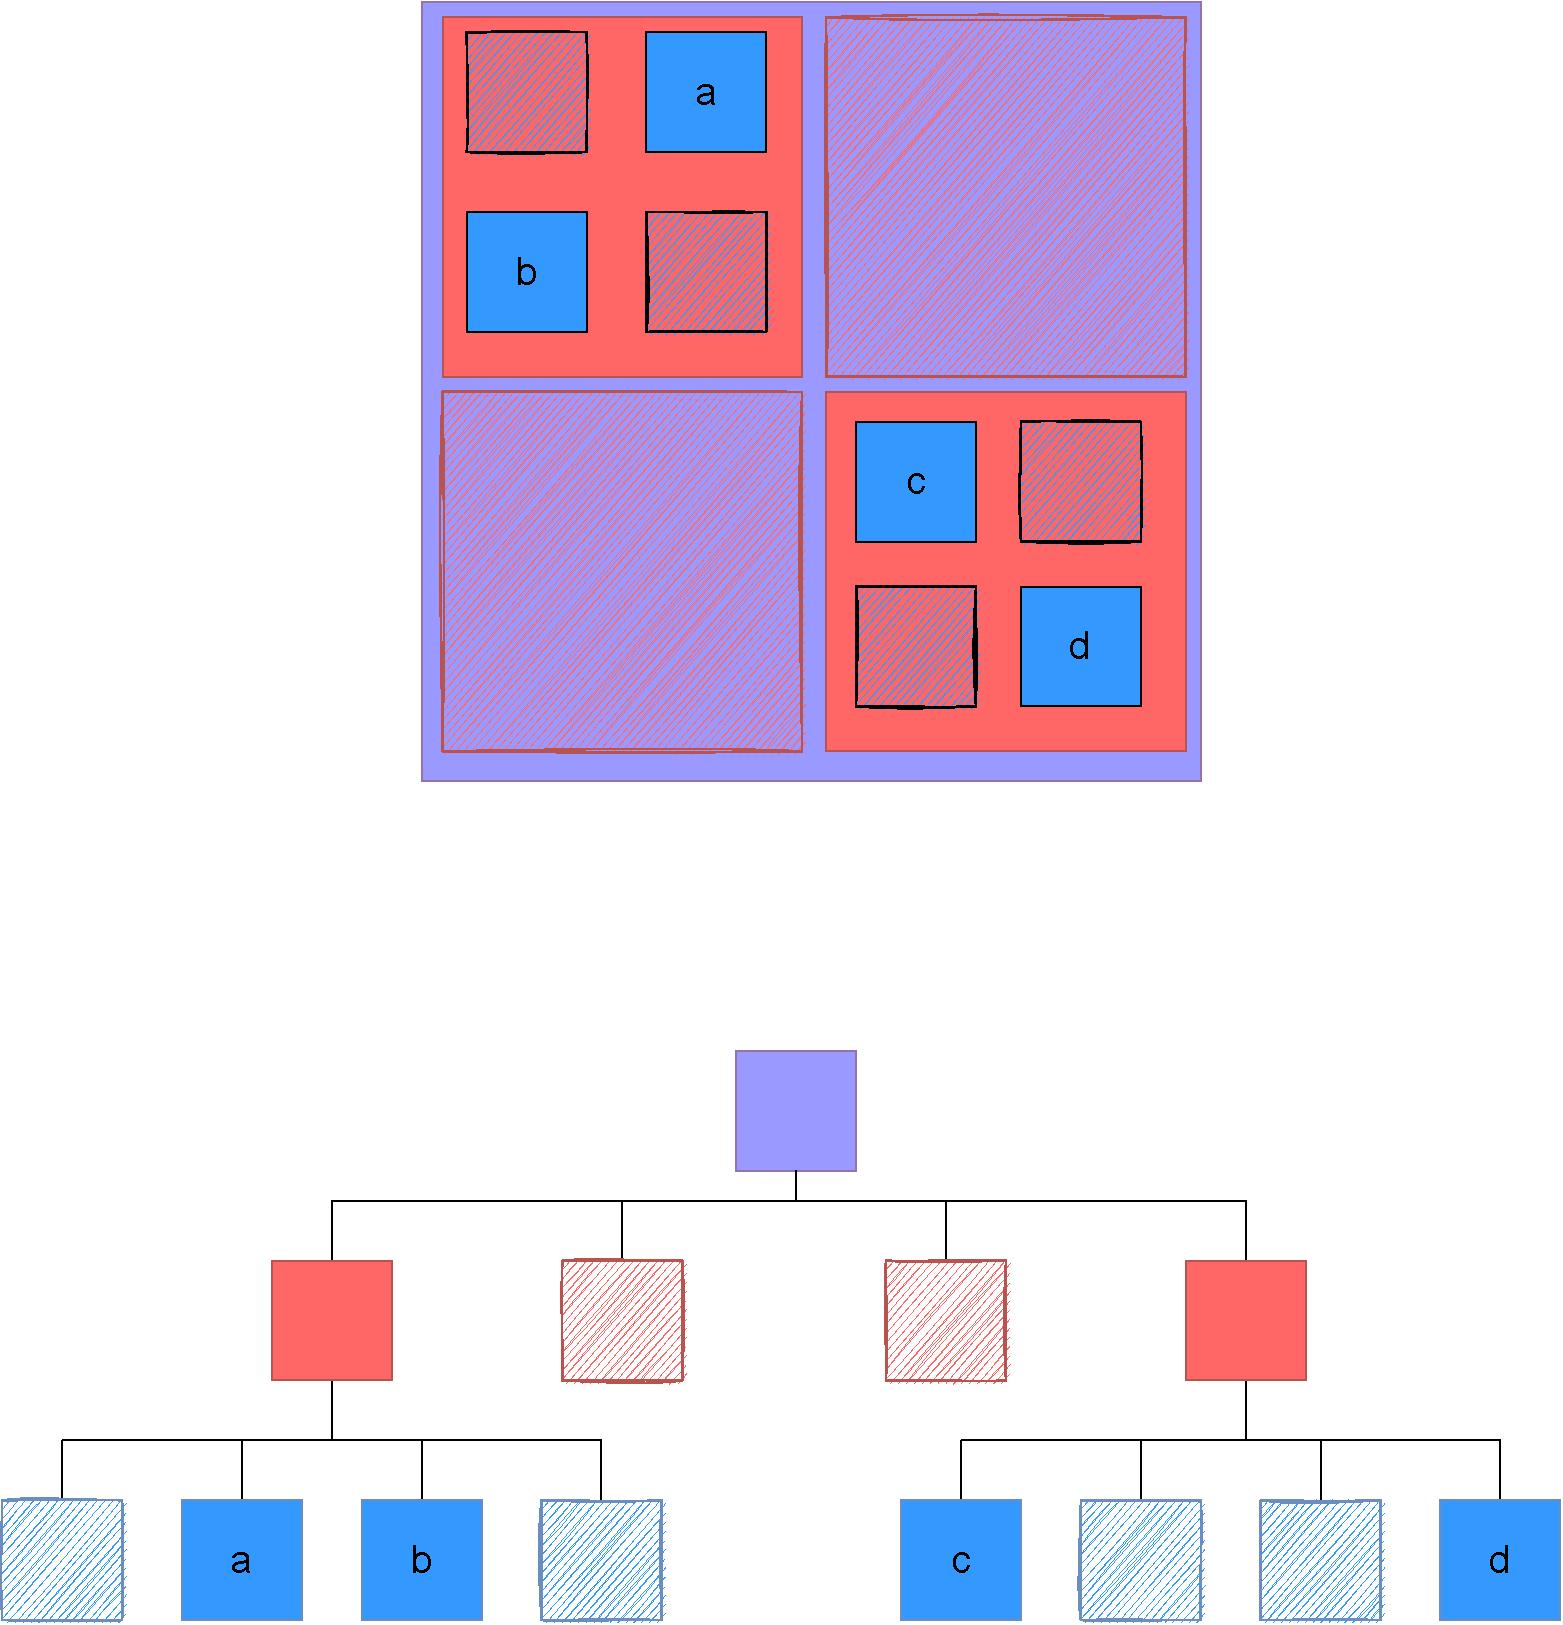
\includegraphics[width=0.8\textwidth]{figures/qtree.drawio.pdf}
    \caption{Quadtree representation}
    \label{fig:qtree}
\end{figure}

\subsection{GRIN}

Some other issues with FHW's frontend exist. FHW uses \textit{external core} representation of GHC, which was removed after GHC 7.6.3. This makes the compiler tightly coupled with Haskell, with the necessity to support various Haskell features, like type classes and burdens of primops. The obsolete version of GHC also makes the development process harder. FHW at the moment does not support partially applied functions in a frontend and CPS transformation is slow.

To mitigate the above issues, we opted for graph reduction intermediate notation  (GRIN)~\cite{GRIN} as a prospective frontend that would tie the frontend of the distiller and dataflow representation. It provides extra optimizations, like heap-points-to analysis, inlining, common subexpression elimination, etc., which improve the results of distillation: the distiller naively inlines some terms duplicating computations. 

All the essential frontend transformations of FHW are actually parts of the translation procedure into GRIN. The procedure includes variable names unification, variable lifting, lambda lifting,  and defunctionalization. These steps were implemented to translate a program from \texttt{.pot} language into \texttt{.grin}. \texttt{.pot} language does not allow recursive let bindings, which makes lambda lifting a bit easier. The algorithm could be found in~\cite{lambda-lift}. Defunctionalization is a part of the GRIN itself: the representation defines \texttt{ap}, \texttt{apply}, and \texttt{eval} procedures. The first one takes a function node and an argument node: it evaluates the function node and applies it to the argument. The second one operates with partially applied functions and constructors: it either saturates a function with one more argument or makes a function call if the argument fully saturates the function. The last one simply evaluates each possible node in a program.  These procedures are built during translation, when either a constructor application, or a function application (partial or saturated) are encountered. The notation is designed for lazy languages: it accumulates nodes without evaluating them if not needed, however the hardware is strict (otherwise, it would be needed to force node evaluation before transferring data from hardware to host). To make translated programs strict, calls to \texttt{eval} procedure are inserted to each function or constructor argument and functions are guaranteed to return and receive pointers to evaluated nodes. The implementation of the translator from \texttt{.pot} to \texttt{.grin} could be found at~\cite{grin-rep}.

GRIN representation uses static single assignment (SSA), and whilst SSA and CPS are equivalent~\cite{ssacps} they are different when generating hardware through dataflow. The current implementation is heavily CPS-depend\-ent, which makes control flow in dataflow straightforward: every recursive call is a tail call. This makes parallelization harder, since otherwise, chained recursive calls could be executed in parallel instead of chaining them with continuations. Such parallelization is more explicit in SSA form. However, SSA conversion into hardware would require heavy modifications to the current dataflow scheme and it is unclear whether it will maintain the existing formalisms that dataflow fulfills. Since CPS is crucial, to express it in GRIN several auxiliary routines are added and existing ones are modified: \texttt{eval} is modified to accept a continuation; \texttt{ap} applies a function to an argument in a continuation, which is passed to function evaluation; \texttt{apCont} is a version of \texttt{ap}, which accepts a continuation; \texttt{applyC} applies a partial function or constructor to an argument with continuation; \texttt{evalC} and \texttt{evalC2} are \texttt{eval} continuations for \texttt{ap} and \texttt{apCont} respectively. A full example for CPS transformation of a program, that adds to zeroes in Peano arithmetics could be seen on GitHub\footnote{\url{https://github.com/Tiltedprogrammer/SparseLinAlgHardware/blob/master/grin-examples/zero_plus_zero.grin} (online; accessed:
2022-06-07) Original program.}\textsuperscript{,}\footnote{\url{https://github.com/Tiltedprogrammer/SparseLinAlgHardware/blob/master/grin-examples/zero_plus_zero.grin.cps} (online; accessed:
2022-06-07) CPS-transformed program.}. 

Unfortunately, it appeared that heap-points-to analysis in the current implementation of GRIN worked only for tiny programs\footnote{\url{https://github.com/grin-compiler/grin/issues/128}  (online; accessed:
2022-06-07) A corresponding issue related to GRIN supporting only small enough programs.}, which is not the case for our sparse linear algebra routines. Since this analysis is crucial in GRIN, the prospective frontend was left until the analysis is performant enough and the part between GRIN and dataflow representation is unimplemented at the moment. 
\section{Memory system}

Initially, FHW did not support passing arguments to the \texttt{main} function, which meant that all matrices were stored in a program's text. It increased the generated circuit size making it unsynthesizable, and did not allow to calculate all overheads, including memory transferring. This section describes a corresponding workaround, namely, it shows the transition from the listing~\ref{lst:main} and how it was implemented at dataflow and hardware levels.

\begin{listing}[b!]
\centering
\begin{minted}{Haskell}
-- How to get from

main :: QTree Bool
main = let m_1 = ...
           m_2 = ... in
       f m_1 m_2
       
-- to
main :: QTree Bool -> QTree Bool -> QTree Bool
main m_1 m_2 = f m_1 m_2



\end{minted}
\caption{Transition to \texttt{main} function with arguments}
\label{lst:main}
\end{listing}

\subsection{Dataflow implementation}

The first step is to compile such programs with \texttt{-fno-do-eta-reduction} GHC flag to prevent GHC from doing \texttt{main = f}, since the \texttt{f} and its mutually recursive functions should be translated as a whole while \texttt{main} function is translated separately. The next step is to enumerate all the arguments to \texttt{main} in order to be able to distinguish the order of arguments of the same type when transferring data. After that, a corresponding fork node is added for each argument that "forks" each argument to the place of its usage, e.g. to the \texttt{f}'s argument.

Memories are implemented as \texttt{bram} nodes in the dataflow. All the writes/reads to the same memory are collected at a corresponding \texttt{merge} actor, which chooses the needed input, and another \texttt{merge} actor chooses whether it is write or read action. The result of read/write is sent to \texttt{demux} node, which routes the result to the caller. A new input to the merge actor is added for each \texttt{main's} argument. Since we do not have any caller in such a case, \texttt{demux}'s output is sent to \texttt{sink} nodes. The only thing that is left is to initialize each memory's pointer. For this purpose, special dataflow \texttt{source} node inputs are added, which initialize memories for each type in \texttt{main}'s arguments, and a \texttt{sink} node is created, which shows the pointer, where the current value is stored at.

\subsection{SystemVerilog implementation}

Modifications from above provided us with three types of \texttt{source} nodes, one to initialize memory pointer, one to provide values to store in memory, and one to finally provide pointers for \texttt{main}'s arguments. These arguments are either scalar values (and, in that case, are not stored in any memory and just flow through dataflow edges) or quadtree node pointers (or quadtree mask pointers). Assuming memory size of $2^{16}$ (it models the situation when data fits into the cache, and currently, FHW supports memory spaces of sizes either $2^8$, $2^{16}$, or $2^{32}$: $2^{16}$ is a tradeoff between matrix sizes and maximum available memory resources on FPGA boards) and that quadtree nodes are represented as the  data type below (\texttt{QError} is needed for error checking), FHW encodes a node in the following manner: first is a valid bit, then an encoding for the node constructor (\texttt{QNone : 00}, \texttt{QVal : 01}, \texttt{QNode : 10}, \texttt{QError : 11}), and then goes either four 16 bit pointers to other nodes (in case the node is \texttt{QNode}) or the encoding for a value (32 bits for integer, for example). For example, \texttt{QVal 4} is encoded as \texttt{0\{61\}100100} (least significant bit is to the right).

\begin{listing}[h!]
\centering
\begin{minted}{Haskell}

data QTree a = QNone 
             | QVal a 
             | QNode (QTree a) (QTree a) (QTree a) (QTree a) 
             | QError;
\end{minted}
\caption{Quadtree data type}
\label{lst:qtree}
\end{listing}

Our trees are complete trees, i.e., every node is saturated (contains four children). To serialize and then deserialize such trees, one stack is sufficient. First, we store reversed post-order tree traversal and pass tree nodes in such order to the corresponding input port of a wrapper for the dataflow module.  We push a pointer for the currently stored node onto the stack (the wrapper takes it from the output port of a \texttt{sink} node added above) then if the input node is \texttt{QNode}, we pop four values from the stack and construct a new \texttt{QNode} with these four pointers in the body, pushing pointer for \texttt{QNode} onto the top. The wrapper then routes this input to the corresponding \texttt{source} node added above. The dataflow network operates under valid/ready protocol, thus we utilize AXI-stream~\cite{axi-stream} protocol to transfer trees into the circuit. The protocol makes it possible to use other predefined blocks in future FPGA design. The wrapper also makes sure that the wrapper's input is of appropriate width for the protocol, extracting the encoded node from more wide representation if needed. The end of each tree is marked with \texttt{tlast}, and the wrapper \texttt{tready} becomes invalid when the last tree arrives (that is why we enumerated the arguments). When all the arguments of all the types arrive, the circuit is finally ready.


\section{Testbench}

This section describes the implementation details of the testbench used to perform benchmarking. One part of the testbench is implemented in System Verilog and another part in \textit{TCL} scripting language, which manages simulation. Also, the section describes a small sparse linear algebra library written in \texttt{.pot} language that we used for experiments.

\subsection{SystemVerilog}

Testbench is a generated module that interacts with the wrapper module by providing appropriate inputs to AXI-stream ports of a wrapper. It reads serialized trees from the given files and sequentially transfers nodes to the wrapper module. The file reading is performed in \texttt{initial block}, so it does not take any simulation time.

The generated dataflow circuit may optionally contain profiling registers for counting the number of memory writes or reads, namely the number of cycles \texttt{write\_enable} is \texttt{1} and read's value is valid and consumer's input is ready. These registers are disabled during synthesis.

\subsection{TCL}

It is not possible to pass arguments to SystemVerilog module during simulation, and for this purpose, TCL language is used since a TCL script in its turn may receive any arguments. The script initializes the project and runs the simulation, providing and gathering values of interest. To modify wire values in SystemVerilog testbench \texttt{set\_value} TCL command is used. It is needed to specify file paths to read the input trees from. Unfortunately, SystemVerilog does not support \texttt{set\_value} for string values, thus all files are enumerated and only file number is set. To collect the information about how long data transferring takes, TCL script uses \texttt{add\_condition} command, which queries the current simulation time on the event occurrence. After the simulation is ended, the script queries current simulation time once again and queries the values of profiling registers. It outputs both time and values to the specified \texttt{.yaml} file. Thus the result of any benchmark is stored completely, which makes a basis for future benchmarks. In a similar manner other tasks could be automated using TCL scripting, e.g., synthesis and resource utilization reporting.



\begin{table}[t!]
\footnotesize
\centering
\begin{tabular}{ |l|l|} 
\hline
\rowcolor{LightBlue}
{Function} & {Description}\\
\hline
\multirow{5}{0.6\textwidth}{\mintinline[fontsize=\scriptsize]{Haskell}{mAdd :: (b->Bool) -> (a->a->b) -> QTree a -> QTree a-> QTree b}} & \multirow{5}{0.35\textwidth}{Performs an arbitrary element-wise operation (passed as the 2nd argument),
between two matrices. The 1st argument defines if the resulting element is zero.
}\\
{} & {}\\
{} & {}\\
{} & {}\\
{} & {}\\
\hline
\multirow{5}{0.6\linewidth}{\mintinline[fontsize=\scriptsize]{Haskell}{mMask :: QTree a -> MQTree -> QTree a}} & \multirow{5}{0.35\linewidth}{Takes a subset specified in the 2nd argument of the elements in the 1st argument. Mask is also represented as a quadtree, nodes just do not store any values.
}\\
{} & {}\\
{} & {}\\
{} & {}\\
{} & {}\\
\hline
\multirow{6}{0.6\linewidth}{\mintinline[fontsize=\scriptsize]{Haskell}{kron :: (b->Bool) -> (a->a->b) -> QTree a -> QTree a -> QTree b}} & \multirow{6}{0.35\linewidth}{Performs Kronecker product of two matrices. The 1st argument defines if the resulting element is zero. The 2nd argument defines the operation applied between an element of the 3rd argument and the 4th argument. 
}\\
{} & {}\\
{} & {}\\
{} & {}\\
{} & {}\\
{} & {}\\
\hline
\multirow{5}{0.6\linewidth}{\mintinline[fontsize=\scriptsize]{Haskell}{map :: (b->Bool) -> (a->b) -> QTree a -> QTree b}} & \multirow{5}{0.35\linewidth}{Applies a function, specified as the 2nd argument to matrix entries from the 3rd argument. The 1st argument defines if the resulting element is zero.
}\\
{} & {}\\
{} & {}\\
{} & {}\\
{} & {}\\
\hline
\end{tabular}
    \caption{Library functions used in evaluation}
    \label{tab:sparse_linalg}
\end{table}

\subsection{Sparse linear algebra library}

We also developed a small library of sparse linear algebra routines in \texttt{.pot} language that we used in our experiments. The library follows the API of GraphBLAS and provides functions for matrix-matrix multiplication, element-wise operations, Kronecker product, \texttt{foldr}s and \texttt{map}s, and masking (i.e. taking a matrix's subset). At the moment, we do not focus on matrix-vector operations, hence our library does not express, e.g., finding all shortest paths. However, the functionality is enough to express other useful algorithms, e.g., triangle counting. The key to expressivity is that \texttt{.pot} is a functional language, thus all the functions are parametric with respect to matrix elements operations.
\texttt{.pot} language does not have any primitives, so passing a matrix could be achieved via emitting Haskell code, or creating a module that contains a proper matrix definition of constructors and importing this module into a program. Such definitions could be obtained via utilities from~\cite{matrix-rep}. Programs could be executed in several ways: by using \texttt{.pot} interpreter, using \texttt{.grin} interpreter, using Haskell emitting, or in hardware simulation.

Function signatures used in the next section are summarized in table~\ref{tab:sparse_linalg}. We choose these functions because we are sure the distiller yields correct and appropriate results for chains of them.
\section{Evaluation}

For performance analysis of proposed solution we evaluated some most common graph algorithms using real-world sparse matrix data. 
As a baseline for comparison we chose LAGraph~\cite{szarnyas2021lagraph} in connection with SuiteSparse~\cite{10.1145/3322125} as a CPU tool, Gunrock~\cite{7967137} and GraphBLAST~\cite{yang2019graphblast} as a Nvidia GPU tools. 
Also, we tested algorithms on several devices with distinct OpenCL vendors in order to validate portability of the proposed solution. 
In general, these evaluation intentions are summarized in the following research questions. 

\vspace{0.2cm}
\begin{itemize}
    \item[\textbf{RQ1}] What is the performance of the proposed solution relative to existing tools for both CPU and GPU analysis?
    
    \item[\textbf{RQ2}] What is the portability of the proposed solution with respect to various device vendors and OpenCL runtimes?
\end{itemize}

\subsection{Evaluation Setup}

For evaluation, we use a PC with Ubuntu 20.04 installed, which has 3.40Hz Intel Core i7-6700 4-core CPU, DDR4 64Gb RAM, and Nvidia GeForce GTX 1070 GPU with 8Gb VRAM. 
Host programs were compiled with GCC 9.3.0 compiler. Programs using CUDA were compiled with GCC 8.4.0 and Nvidia NVCC 10.1.243 compiler.
Release mode and maximum optimization level was enabled for all tested programs. 
Data loading time, preparation, format transformations and host-device initial communications are excluded from time measurements. 
All tests are averaged across 10 runs.
Additional warm-up run for each test execution is excluded from measurements.

\subsection{Graph Algorithms}

For preliminary study \textit{breadth-first search} (bfs) and \textit{triangles counting} (tc) algorithms were chosen, since they allows analyse the performance of \textit{vxm} and \textit{mxm} operations, rely heavily on \textit{masking}, and utilize \textit{reduction} or \textit{assignment}. 
BFS implementation utilizes automated vector storage from sparse to dense switch and only \textit{}{push optimization}. 
TC implementation uses masked \textit{mxm} of source lower-triangular matrix with second transposed argument.

\subsection{Dataset}

Nine graph matrices were selected from the Sparse Matrix Collection at University of Florida~\cite{dataset:10.1145/2049662.2049663}. 
Information about graphs is summarized in Table~\ref{dataset:info}. 
All datasets are converted to undirected graphs. 
Self-loops and duplicated edges are removed.

\begin{table}[htbp]
\caption{Dataset description.} 
\begin{center}
    \rowcolors{2}{black!2}{black!10}
    \begin{tabular}{|l|r|r|r|}
    \hline
    Dataset & Vertices  & Edges & Max Degree \\
    \hline
    \hline
    coAuthorsCiteseer & 227.3K &   1.6M &    1372 \\
    coPapersDBLP      & 540.4K &  30.4M &    3299 \\
    hollywood-2009    &   1.1M & 113.8M &  11,467 \\
    roadNet-CA        &   1.9M &   5.5M &      12 \\
    com-Orkut         &     3M &   234M &   33313 \\
    cit-Patents       &   3.7M &  16.5M &     793 \\
    rgg\_n\_2\_22\_s0 &   4.1M &  60.7M &      36 \\
    soc-LiveJournal   &   4.8M &  68.9M &  20,333 \\
    indochina-2004    &   7.5M & 194.1M & 256,425 \\
    \hline
    \end{tabular}
    \label{dataset:info}
\end{center}
\end{table}

\subsection{Results}

Table~\ref{results} presents results of the evaluation and compares performance of Spla against other tool on different execution platforms.
Tools are grouped by the type of the device for the execution, where either Nvidia GPU or Intel CPU are used. 
Cell left empty if tested tool failed to analyse graph due to \textit{out of memory} exception.

In general, Spla BFS shows acceptable performance, especially on graphs with large vertex degree, such as soc-LiveJournal and com-Orkut.
On graphs roadNet-CA and rgg it has a significant performance drop due to the nature of underlying algorithms and data structures. 
Firstly, library utilizes immutable data buffers. Thus, iteratively updated dense vector of reached vertices must be copied for each modification, what dominates the performance of the library on a graph with large search depth. 
Secondly, Spla BFS does not utilise \textit{pull optimization}, what is critical in a graph with relatively small search frontier. 

Spla TC has a good performance on GPU, which is better in all cases that reference SuiteSparse solution. 
But in most tests GPU competitors, especially Gunrock, show smaller processing times. 
GraphBLAST shows better performance as well. 
Library utilises masked SpGEMM algorithm, the same as in GraphBLAST, but without \textit{identity} element to fill gaps. 
Library explicitly stores all non-zero elements, and uses mask to reduce only non-zero while evaluating dot products of rows and columns. 
What causes extra divergence inside work groups. 
On Intel device Spla shows better performance compared to SuiteSparse on com-Orkut, cit-Patents and soc-LiveJournal. 
A possible reason is the large lengths of processed rows and columns in the product of matrices.

Gunrock shows nearly best average performance due to its specialized and optimized algorithms.
Also, it has good time characteristics on a mentioned earlier roadNet-CA and rgg in BFS algortihm. 
GraphBLAST follows Gunrock and show good performance as well. 
But it runs out of memory on a two significantly large graphs con-Orkut and indochina-2004. 
Spla does not rut out of memory on any test due to simplified storage scheme.

\begin{table}[htbp]
\caption{Graph algorithms evaluation results.\\Time in milliseconds (lower is better).} 
\begin{center}
    \begin{tabular}{|l|r|r|r|r|r|}
    \hline
    \multirow{2}{*}{Dataset} & \multicolumn{3}{c|}{Nvidia} & \multicolumn{2}{c|}{Intel} \\
    \cline{2-6}
    & GR & GB & SP & SS & SP \\
    \hline
    \hline
    \multicolumn{6}{|c|}{BFS} \\
    \hline
    \rowcolor{black!10} hollywood-2009    &  20.3 &  82.3 &   36.9 &   23.7 &   303.4 \\
    \rowcolor{black!2 } roadNet-CA        &  33.4 & 130.8 & 1456.4 &  168.2 &   965.6 \\
    \rowcolor{black!10} soc-LiveJournal   &  60.9 &  80.6 &   90.6 &   75.2 &  1206.3 \\
    \rowcolor{black!2 } rgg\_n\_2\_22\_s0 &  98.7 & 414.9 & 4504.3 & 1215.7 & 15630.1 \\
    \rowcolor{black!10} com-Orkut         & 205.2 & -- -- &  117.9 &   43.2 &   903.6 \\
    \rowcolor{black!2 } indochina-2004    &  32.7 & -- -- &  199.6 &  227.1 &  2704.6 \\
    \hline
    \hline
    \multicolumn{6}{|c|}{TC} \\
    \hline
    \rowcolor{black!10} coAuthorsCiteseer &   2.1 &    2.0 &    9.5 &    17.5 &    64.9 \\
    \rowcolor{black!2 } coPapersDBLP      &   5.7 &   94.4 &  201.9 &   543.1 &  1537.8 \\
    \rowcolor{black!10} roadNet-CA        &  34.3 &    5.8 &   16.1 &    47.1 &   357.6 \\
    \rowcolor{black!2 } com-Orkut         & 218.1 & 1583.8 & 2407.4 & 23731.4 & 15049.5 \\
    \rowcolor{black!10} cit-Patents       &  49.7 &   52.9 &   90.6 &   698.3 &   684.1 \\
    \rowcolor{black!2 } soc-LiveJournal   &  69.1 &  449.6 &  673.9 &  4002.6 &  3823.9 \\
    \hline
    \hline
    \multicolumn{6}{l}{Tools: Gunrock (GR), GraphBLAST (GB), SuiteSparse (SS), Spla (SP).} \\
    \end{tabular}
    \label{results}
\end{center}
\end{table}
 
% Two GPU

% \begin{table}[htbp]
%     \caption{Table Type Styles}
%     \begin{center}
%     \begin{tabular}{|c|c|c|c|}
%     \hline
%     \textbf{Table}&\multicolumn{3}{|c|}{\textbf{Table Column Head}} \\
%     \cline{2-4} 
%     \textbf{Head} & \textbf{\textit{Table column subhead}}& \textbf{\textit{Subhead}}& \textbf{\textit{Subhead}} \\
%     \hline
%     copy& More table copy$^{\mathrm{a}}$& &  \\
%     \hline
%     \multicolumn{4}{l}{$^{\mathrm{a}}$Sample of a Table footnote.}
%     \end{tabular}
%     \label{tab2}
%     \end{center}
% \end{table}

\clearpage
\section{Related Work}

This section will try to show more clearly the place the work takes among adjacent works.

Firstly, the work utilizes distillation technique to provide automatic fusion of sparse linear algebra routines. At the moment, we are not aware of other works that focus on sparse linear algebra routines fusion from implementation perspective. However, it is worth noticing that SuiteSparse addresses this problem in future work~\cite{newsuitesparse}. The approaches that work well for dense routines fusion struggle with index arithmetic, e.g.~\cite{Futhark}, induced by sparse representation. Other approaches makes specific assumption about the operands or require to express computations with the help of combinators~\cite{StreamFus}. Our approach makes no assumptions and was shown to work successfully.

Secondly, in contrast with other works, e.g.\cite{zhang2020sparch}, this work opts for functional high-level synthesis to produce hardware. Thus, we are not limited to only specific kernels like matrix-vector multiplication. FHW is not the only functional high-level synthesis compiler, however, it appeared to be the best fit for our pipeline. A more detailed discussion of alternatives could be found at~\cite{Edwards2019FHWP}. Although we have slightly worse performance than software counterparts, the approach has a certain potential. For the same reason, we do not provide any comparison with other hardware works at the moment. Also, they are too specialized, e.g. they provide only matrix multiplication operations, while we focus on providing a reasonable GraphBLAS subset.

Finally,~\cite{superreduceron} evaluates whether supercompilation makes any benefits when a functional program is executed on a dedicated reduction-based processor \textit{Reduceron}. Unlike this work, we use another hardware backend, distillation, and choose specific programs, namely those that contain sparse linear algebra routines. However, we plan to perform the same evaluation with Reduceron as a backend.
\section{Conclusion}

In this paper we present a library for sparse Boolean linear algebra which implements such basic operations as matrix-matrix multiplication and element-wise matrix-matrix addition in both Cuda and OpenCL.
Evaluation shows that our Boolean-specific implementations faster and require less memory than generic, not the Boolean optimized, operations from state-of-the-art libraries. 
Thus, the specialization of operations for this data type makes sense. 

The first direction of the future work is to integrate all parts (OpenCL and Cuda backends) into a single library and improve its documentation and prepare to publish.
Moreover, it is necessary to extend the library with other operations, including matrix-vector operations, masking, and so on.
As a result a Python package should be published.

Another important step is to evaluate the library on different algorithms and devices.
Namely, algorithms for RPQ and CFPQ should be implemented and evaluated on related data sets.
Also, it is necessary to evaluate OpenCL version on FPGA which may require additional technical effort and code changes.

Finally, we plan to discuss with GraphBLAS community possible ways to use our library as a backend for GraphBLAST or SuiteSparse in case of Boolean computations.
Moreover, it may be possible to use implemented algorithms as a foundation for generalization to arbitrary semirings.


\setmonofont[Mapping=tex-text]{CMU Typewriter Text}
  \bibliographystyle{ugost2008ls}
  \bibliography{vkr}
\end{document}
